\documentclass[10pt]{article}
\PassOptionsToPackage{table}{xcolor}
\usepackage[preprint]{tmlr}
% \usepackage{tmlr}            % anonymous TMLR submission
% \usepackage[accepted]{tmlr}  % camera-ready

\usepackage{amsmath,amssymb,amsthm,mathtools}
\usepackage{graphicx}
\usepackage{enumitem}
\usepackage{hyperref}
\usepackage{cleveref}
\usepackage{booktabs}
\usepackage{xcolor}
\usepackage{float}
\usepackage{caption}

\newtheorem{theorem}{Theorem}[section]
\newtheorem{proposition}[theorem]{Proposition}
\newtheorem{lemma}[theorem]{Lemma}
\newtheorem{corollary}[theorem]{Corollary}
\theoremstyle{definition}
\newtheorem{definition}[theorem]{Definition}
\theoremstyle{remark}
\newtheorem{remark}[theorem]{Remark}

\newcommand{\R}{\mathbb{R}}
\newcommand{\xstate}{\mathbf{x}}

\title{An Effective-Rank Audit of Alignment-Induced\\
  Activation Shifts: Confound Control, Constructive\\
  Calibration, and Limits}

\author{\name Yuki Nakamura \\
        \addr The Open University of Japan \\
        \addr ORCID: \texttt{\href{https://orcid.org/0009-0001-7174-6737}{0009-0001-7174-6737}}}

\begin{document}
\maketitle

\begin{abstract}
We audit alignment-induced shifts in residual-stream
activations of three open-weight instruction-tuned LLMs
(Llama-3.1-8B-Instruct, Gemma-2-9B-it,
Qwen-2.5-7B-Instruct) using the effective rank of the
alignment modification matrix on safety-relevant inputs,
$\rho_{\epsilon} :=
\operatorname{rank}_{\epsilon}(M_{\mathcal{D}_s})/d$,
which formalizes the single-refusal-direction
observation of \citet{arditi2024refusal} as a continuous
quantity.  The paper has three contributions.
\textbf{(1) Confound-controlled measurement.}  A
four-variant decomposition of the modification matrix
($M_{\mathrm{naive}}, M_{\mathrm{template}},
M_{\mathrm{aligned}}, M_{\mathrm{DiD}}$) separates the
contributions of chat-template formatting, alignment-stage
shift, and the refusal-mediating direction, and recovers
the Arditi
refusal direction on $M_{\mathrm{DiD}}$ at
$|\cos|\in\{0.77, 0.86, 0.50\}$ (Llama/Gemma/Qwen),
while $M_{\mathrm{template}}$ gives chat-template-controlled
$\rho_{\epsilon}\in\{0.0029, 0.0048, 0.0044\}$; the
centered SVD residual is $4$--$7\times$ larger,
indicating the headline rank is dominated by a single
mean direction.
\textbf{(2) Constructive calibration with a sweet-spot
vs.\ brittle distinction.}  On a 3-layer MLP across
$\rho_{\epsilon}\in\{0.008, 0.17, 0.33, 0.40\}$, high
$\rho_{\epsilon}$ via mild rank-maximization
regularization ($\lambda=5$) buys ablation robustness
($\geq 0.97$ compliance through projection of $62.5\%$
of the representation), while strong regularization at
the same nominal $\rho_{\epsilon}$ ($\lambda=50$) does
not ($0.10$ at $r=40$).  $\rho_{\epsilon}$ is therefore
a diagnostic for fragility, not a target whose
mechanical inflation buys robustness.  Linear-projection
fragility (Prop.~\ref{prop:fragility}, unconditional)
and an $O(\rho_{\epsilon}d)$ achievability bound on
faking footprint (Prop.~\ref{prop:faking},
representational only) are the two structural
consequences of low $\rho_{\epsilon}$.
\textbf{(3) Limits of rank-based diagnostics.}
(a) The diagnostic is not safety-specific (LRH baseline
$\rho_{\epsilon}\approx 0.008$--$0.010$, only
$2$--$3\times$ the safety value); (b) SVD principal
ordering does not match causal ordering (Llama
narrow-band $u_2$ ranks second by $\sigma$ but is
causally inert; cumulative ablation is non-monotone at
$k{=}5$); (c) the spectral-gap hypothesis required to
upgrade Prop.~\ref{prop:faking}'s achievability to a
matching $\Omega(\rho_{\epsilon}d)$ Mirsky-route lower
bound fails empirically ($\kappa_{\mathrm{emp}}>8$ on
$1/90$ Llama layer-reference pairs and $0/36$ MLP
combinations) and structurally
(Lemma~\ref{lem:kappa_obstruction}:
$\kappa_{\mathrm{lb}}\leq 2/(\epsilon r)$, so the
hypothesis $\kappa>8$ fails once $\epsilon r > 1/4$).
The matching lower bound remains an open problem
(\S\ref{sec:open}).
\end{abstract}


% ============================================================================
\section{Introduction}
\label{sec:intro}
% ============================================================================

\citet{arditi2024refusal} showed refusal in
instruction-tuned LLMs is mediated by a single
direction in activation space, and that ablating that
direction removes safety entirely.  This is a striking
empirical observation about the geometry of current
alignment: the shift between pre-trained and aligned
activations on safety-relevant inputs lives in a small
number of directions, and a sub-capable adversary with
a truncated SVD can identify and remove them.

This paper audits the structural consequences of that
observation by formalizing it as a continuous quantity.
Let $M_{\mathcal{D}_s} := [h_{\mathrm{align}}(x_i) -
h_{\mathrm{pre}}(x_i)]_i$ be the paired alignment
modification at a fixed layer over a safety-relevant
input distribution $\mathcal{D}_s$.  The
\emph{separability index} is
\[
  \rho_{\epsilon}
  \;:=\;
  \operatorname{rank}_{\epsilon}(M_{\mathcal{D}_s})/d
\]
(\S\ref{sec:two_modes}), the effective rank of
$M_{\mathcal{D}_s}$ normalized by the representation
dimension.  On Llama-3.1-8B-Instruct, Gemma-2-9B-it,
and Qwen-2.5-7B-Instruct the chat-template-controlled
$\rho_{\epsilon}$ is $0.0029, 0.0048, 0.0044$; the
centered SVD residual is $4$--$7\times$ larger than the
uncentered, so the index is dominated by a single mean
direction that aligns with the Arditi refusal direction
at high cosine after control-distribution subtraction.
The paper makes three contributions.

\paragraph{Contribution 1: confound-controlled measurement.}
A four-variant decomposition of the modification
matrix
($M_{\mathrm{naive}}, M_{\mathrm{template}},
M_{\mathrm{aligned}}, M_{\mathrm{DiD}}$;
\S\ref{sec:diagnosis_setup}) separates the
contributions of chat-template formatting, the
alignment-stage shift, and the refusal-mediating
direction.  The
chat-template-controlled $M_{\mathrm{template}}$ is the
cleanest quantity for the separability index;
$M_{\mathrm{DiD}}$ subtracts the control column-mean
and recovers Arditi's intra-aligned refusal direction
at $|\cos|\in\{0.77, 0.86, 0.50\}$ (Llama, Gemma,
Qwen), high in Llama and Gemma, moderate in Qwen---the
Arditi rank-$1$ collapse is not universal but holds on
two of three families.  $M_{\mathrm{template}}$ and
$M_{\mathrm{DiD}}$ measure structurally different
quantities (alignment-stage shift vs.\ refusal-mediating
direction); the four-variant view makes the distinction
explicit and locates the chat-template confound that
inflates uncontrolled $\rho_{\epsilon}$ estimates by
${\approx}4\times$ (App.~\ref{app:four_variants}).

\paragraph{Contribution 2: constructive calibration with
a sweet-spot vs.\ brittle distinction.}
On a 3-layer MLP across $\rho_{\epsilon} \in \{0.008,
0.17, 0.33, 0.40\}$
(\S\ref{sec:calibration},
App.~\ref{app:calibration_v2_ablation}), high
$\rho_{\epsilon}$ via mild rank-maximization
regularization ($\lambda=5$, baseline compliance $0.86$)
buys ablation robustness ($\geq 0.97$ compliance
through projection of $62.5\%$ of the representation),
while strong regularization at the same nominal
$\rho_{\epsilon}$ ($\lambda=50$, baseline compliance
$0.71$) does not (post-ablation compliance $0.10$ at
$r=40$).  $\rho_{\epsilon}$ is therefore a
\emph{diagnostic}; mechanical rank inflation via stronger
regularization does not buy structural robustness, so
treating $\rho_{\epsilon}$ as an optimization target
fails on the calibration testbed.
Two structural consequences of low $\rho_{\epsilon}$
support the diagnostic interpretation:
linear-projection fragility
(Prop.~\ref{prop:fragility}, unconditional) and an
$O(\rho_{\epsilon}d)$ achievability bound on faking
footprint
(Prop.~\ref{prop:faking}, representational only).  The
matching $\Omega(\rho_{\epsilon}d)$ lower bound, which
would make low $\rho_{\epsilon}$ a structural
\emph{condition} for fake-resistant safety, is left as
an open problem (\S\ref{sec:open}).

\paragraph{Contribution 3: limits of rank-based
diagnostics.}
We document three.  \textbf{(a) Not safety-specific.}
The LRH baseline (App.~\ref{app:lrh}) gives arbitrary
linear concepts $\rho_{\epsilon} \approx 0.008$--$0.010$
in the same models, only $2$--$3\times$ the safety
value: low rank is a generic property of post-training
linear concepts, and the bridge from rank to behavior
is supplied by causal ablation (Test~2,
\S\ref{sec:diagnosis_ablation}), not by the rank number.
\textbf{(b) SVD ordering does not match causal
ordering.}  On Llama narrow-band, $u_2$ ranks second by
squared variance but has near-zero causal effect
on refusal under projection ablation; cumulative
top-$k$ ablation is non-monotone at $k=5$
(Table~\ref{tab:perdir_llama_body},
\S\ref{sec:diagnosis_ablation}).  Behavioral fragility
must be measured directly by Test~2, not read off the
SVD spectrum.
\textbf{(c) The spectral-gap hypothesis required for the
Mirsky lower-bound sketch fails.}  We measure
$\kappa_{\mathrm{emp}}$ across three publicly available
unsafe-mode references for Llama (\S\ref{sec:open},
App.~\ref{app:kappa}): $\kappa_{\mathrm{emp}}>8$ on
$1/90$ layer-reference pairs.  In a controlled MLP
sweep (App.~\ref{app:calibration_kappa}), $0/36$
honest--unsafe combinations cross the threshold, with
the worst case in the distributed-vs-distributed regime
the high-$\rho_{\epsilon}$ regime targets.  We
identify a geometric reason
(Lemma~\ref{lem:kappa_obstruction}:
$\kappa_{\mathrm{lb}}\leq 2/(\epsilon r)$) that
$\kappa>8$ is structurally hard to satisfy whenever the
modal-difference signal has non-trivial effective rank.

The diagnostic is computable by a verifier strictly
weaker than the diagnosed system, given whitebox
paired checkpoints and a fixed $\mathcal{D}_s$
(Remark~\ref{rem:bootstrap}); the capability burden is
displaced onto constructing $\mathcal{D}_s$, not
removed.


% ============================================================================
\section{The Separability Index}
\label{sec:two_modes}
% ============================================================================

Let $f_{\mathrm{pre}}, f_{\mathrm{align}}$ be the
pre- and post-alignment systems, $h_{\mathrm{pre}}(x),
h_{\mathrm{align}}(x) \in \mathbb{R}^d$ their layer
activations, and $\mathcal{D}_s, \mathcal{D}_c$
distributions of safety-relevant and control inputs.
The alignment modification matrix on a sample
$x_1,\ldots,x_n \sim \mathcal{D}$ is
\begin{equation}
  M_{\mathcal{D}}
  \;:=\;
  \bigl[\,
    h_{\mathrm{align}}(x_1) - h_{\mathrm{pre}}(x_1),
    \ldots,
    h_{\mathrm{align}}(x_n) - h_{\mathrm{pre}}(x_n)
  \,\bigr]
  \;\in\; \mathbb{R}^{d \times n}.
  \label{eq:modification}
\end{equation}
With singular values $\sigma_1 \geq \sigma_2 \geq \cdots
\geq 0$ of $M_{\mathcal{D}}$, the \emph{effective rank}
at tolerance $\epsilon_{\mathrm{rank}} \in (0,1)$ is
\begin{equation}
  \operatorname{rank}_{\epsilon_{\mathrm{rank}}}(M_{\mathcal{D}})
  := \min\bigl\{\, k :
    \textstyle\sum_{i=1}^{k} \sigma_i^2
    \,\geq\, (1 - \epsilon_{\mathrm{rank}})
    \textstyle\sum_i \sigma_i^2 \bigr\}.
  \label{eq:effrank}
\end{equation}
We write $\epsilon$ when unambiguous and reserve
$\epsilon_{\mathrm{pert}}$ for the perturbation-norm
tolerance in \S\ref{sec:open}.  We use
$\epsilon_{\mathrm{rank}} = 0.05$.  Since
$M_{\mathcal{D}} \in \mathbb{R}^{d\times n}$ has rank
$\leq \min(d, n)$, when $n < d$ the sample-relative
ratio $\operatorname{rank}_{\epsilon}/\min(d, n)$ is
the more conservative summary; \S\ref{sec:diagnosis}
reports both and sweeps $n$.

The question is not whether $f_{\mathrm{align}}$
produces safer outputs (assumed) but how the
modification is distributed in representation space.

\subsection{Separable Safety}
\label{sec:constraint}

\begin{definition}[Separable Safety]
\label{def:separable}
An alignment procedure produces
\emph{$(k, \epsilon)$-separable safety} on safety-relevant
distribution $\mathcal{D}_s$ if the alignment modification
is concentrated in a low-dimensional subspace:
\begin{equation}
  \operatorname{rank}_{\epsilon}(M_{\mathcal{D}_s})
  \;\leq\; k,
  \qquad k \ll d.
  \label{eq:separable}
\end{equation}
Equivalently, the top-$k$ principal components of
$M_{\mathcal{D}_s}$ capture at least a
$(1-\epsilon)$-fraction of the modification's variance.
Safety is \emph{perfectly separable} when the alignment
shift is rank-one
($\operatorname{rank}_{\epsilon}(M_{\mathcal{D}_s}) = 1$
for small $\epsilon$).
\end{definition}

Separability is a statement about the \emph{readout}
of the alignment modification at the residual stream,
consistent with arbitrarily complex internal computation
producing the readout (Remark~\ref{rem:readout_vs_mechanism}).

\begin{remark}[Modification Level vs Mechanism]
\label{rem:readout_vs_mechanism}
$M_{\mathcal{D}_s}$ records what alignment changes at
the readout, not the internal computation that produced
the change.  Mechanistic interpretability~\citep{olah2020zoom,
arditi2024refusal, wollschlager2025} consistently finds
distributed non-linear computations writing into
low-dimensional residual subspaces; our diagnostic is
sensitive to that readout structure and silent on the
depth of computation.  Fragility, fakeability, and
verifiability claims thus concern residual-stream attacks
(projection, steering, mode-toggling), not arbitrary
adversarial pressure on the mechanism.
\end{remark}

\begin{remark}[Linear Recoverability]
\label{rem:recoverability}
Low rank means a rank-$k$ projection $P$ recovers
$(1-\epsilon)$-energy on $P$ and removes it on $I-P$;
a linear probe with $\leq k$ features achieves
near-perfect aligned-vs-pre-trained classification when
the shift exceeds activation noise.  Non-linear probes
may find additional structure outside SVD.
\end{remark}

Low $\rho_{\epsilon}$ has one unconditional geometric
consequence (Prop.~\ref{prop:fragility}: a rank-$k$
projection removes $(1-\epsilon)$-variance) and one
unconditional representational consequence
(Prop.~\ref{prop:faking}: an $O(\rho_{\epsilon}d)$
faking footprint is achievable).  Whether the
representational fragility translates to behavioral
fragility, and whether the achievability has a matching
$\Omega$ lower bound, are separate empirical
(\S\ref{sec:diagnosis_ablation}) and open-problem
(\S\ref{sec:open}) questions.


\subsection{The Separability Spectrum}
\label{sec:nature}

The \emph{separability index} is
\begin{equation}
  \rho_{\epsilon}(M_{\mathcal{D}_s})
  := \operatorname{rank}_{\epsilon}(M_{\mathcal{D}_s}) / d
  \in (0, 1].
  \label{eq:sep_index}
\end{equation}
At $\rho_{\epsilon} \ll 1$ the modification inherits
fragility and low-cost-faking (\S\ref{sec:consequences});
at $\rho_{\epsilon} \to 1$ alignment spans the full
representation (constructing such an LLM alignment
is open).

$\rho_{\epsilon}$ is structural, not behavioral: two
systems with identical $\mathcal{D}_s$ compliance can
have very different $\rho_{\epsilon}$
(\S\ref{sec:calibration}).  Its diagnostic content is
projection-ablation response, not nominal behavior.


% ============================================================================
\section{Consequences of Separability}
\label{sec:consequences}
% ============================================================================

The diagnostic carries one geometric implication
unconditionally; behavioral and converse-direction
implications require additional structure that this
paper shows is not free (\S\ref{sec:open}).

\subsection{Fragility}
\label{sec:fragility}

\begin{proposition}[Linear Fragility]
\label{prop:fragility}
If alignment is $(k,\epsilon)$-separable on $\mathcal{D}_s$,
an adversary with whitebox activation access and the
pre-trained baseline can, given a finite sample
sufficient to estimate the top-$k$ principal subspace
(empirically $n{=}200$ suffices on $d{\geq}3584$;
see App.~\ref{app:bootstrap} for bootstrap stability checks and
App.~\ref{app:n_sweep} for sample-size sensitivity),
remove $(1-\epsilon)$-variance by a rank-$k$ projection.
\end{proposition}

\begin{proof}
$M_{\mathcal{D}_s} = U \Sigma V^\top$, $U_k$ the top-$k$
left singular vectors, $P_k := U_k U_k^\top$.
$(k,\epsilon)$-separability gives $\sum_{i\leq k}\sigma_i^2
\geq (1-\epsilon)\sum_i \sigma_i^2$.  Replace
$h_{\mathrm{align}}(x)$ with $(I-P_k) h_{\mathrm{align}}(x)
+ P_k h_{\mathrm{pre}}(x)$.  $U_k$ from a truncated SVD
on a sample.
\end{proof}

\begin{remark}[Threat Model]
\label{rem:threat_model}
Substitution requires open-weight access to
$h_{\mathrm{pre}}$.  The weaker form
$h_{\mathrm{align}} \to (I-P_k) h_{\mathrm{align}}$
needs no such access but only shows the principal
subspace is causally privileged; \S\ref{sec:diagnosis}
uses the weaker form.  LoRA fine-tuning and prompt
jailbreaks are out of scope.
\end{remark}

\paragraph{Geometric vs.\ behavioral fragility.}
SVD orders by variance, not causal authority: in
Llama narrow band $u_2$ has near-zero causal
effect despite ranking second by $\sigma$
(Table~\ref{tab:perdir_llama_body}).  Test~2
(\S\ref{sec:diagnosis_ablation}) is the bridge: in
Gemma narrow $k=3$ the principal and causal subspaces
coincide; in Llama they don't.  We do not state a
behavioral-fragility proposition---no Lipschitz
hypothesis holds on the principal parametrization, and
a causal-subspace hypothesis is empirically circular.

\begin{remark}[$k=1$ and Arditi]
\label{rem:k1_arditi}
At $\operatorname{rank}_{\epsilon}\approx 1$, $u_1$
coincides with $\bar{\Delta} = \mathbb{E}[h_{\mathrm{align}}
- h_{\mathrm{pre}}]$.  \citet{arditi2024refusal}'s
direction is the distinct within-aligned quantity
$\bar{\Delta}^{\mathrm{Arditi}} =
\mathbb{E}_{\mathcal{D}_s}[h_{\mathrm{align}}] -
\mathbb{E}_{\mathcal{D}_c}[h_{\mathrm{align}}]$.
Cosines in \S\ref{sec:diagnosis}.
\end{remark}

\begin{remark}[Computability by a sub-capable verifier]
\label{rem:bootstrap}
$\rho_{\epsilon}$ is computable by truncated SVD on
paired-checkpoint activations alone.  The capability
burden is displaced onto $\mathcal{D}_s$, not removed:
a super-capable system can produce safety-relevant
inputs humans cannot recognize, and a system optimized
on $\mathcal{D}_s$ may look safe outside it.
\end{remark}

\subsection{Cost of Faking: Achievability}
\label{sec:faking_achievability_body}

Fragility (\S\ref{sec:fragility}) says low
$\rho_{\epsilon}$ \emph{permits} an adversary to
project out the alignment shift.  A symmetric question
about \emph{faking} alignment---can a deceptive policy
exhibit honest activations under monitoring while
behaving differently when unmonitored---has the same
representational-footprint upper bound, also
unconditional.

\begin{proposition}[Representational Achievability]
\label{prop:faking}
Let $r := \operatorname{rank}_{\epsilon}(M^{\mathrm{honest}}_{\mathcal{D}_s})$
and $P_r$ the projector onto its top-$r$ principal
subspace.  The mode-toggling policy
$h^{(m)}(x) = h_{\mathrm{pre}}(x) + m \cdot
P_r(h_{\mathrm{align}}(x) - h_{\mathrm{pre}}(x))$,
$m\in\{0,1\}$, matches the projected honest shift
$P_r M^{\mathrm{honest}}_{\mathcal{D}_s}$ in monitored
mode and has rank-$r$ modal difference: representational
footprint $O(\rho_{\epsilon}\,d)$.  (Proof in
App.~\ref{app:faking_achievability}.)
\end{proposition}

The statement is unconditional but weak: it says low
$\rho_{\epsilon}$ \emph{permits} a representationally-cheap
shift matching the projected honest activations on
$\mathcal{D}_s$, not a policy that passes any non-trivial
behavioral monitor.  The matching $\Omega(\rho_{\epsilon}d)$
lower bound---which would yield the contrapositive
``high $\rho_{\epsilon}$ blocks low-cost
mode-toggling''---is left as an open problem
(\S\ref{sec:open}); a natural Mirsky-style sketch
requires a spectral-gap hypothesis we show fails both
empirically and structurally.


% ============================================================================
\section{The Three Diagnostic Tests}
\label{sec:verification}
% ============================================================================

Three tests on $\mathcal{D}_s$ at a chosen layer band:
\textbf{Test~1 (rank)}: SVD on $M_{\mathcal{D}_s}$,
report $\operatorname{rank}_{\epsilon}$ at
$\epsilon=0.05$ ($\mathcal{D}_c$ as control).
\textbf{Test~2 (causal ablation)}: project out
$P_k = U_k U_k^\top$, measure refusal change vs.\ a
random rank-$k$ null.
\textbf{Test~3 (principal alignment)}:
$|\cos(u_1, \bar{\Delta})|$ on $\mathcal{D}_s$.

Low $\rho_{\epsilon}$ predicts (T1) steeply rising
cumulative variance, (T2) sharp refusal collapse on
principal-but-not-random ablation, (T3) high cosine.
Test~2 is the empirical bridge: SVD ordering does not
match causal ordering globally
(\S\ref{sec:diagnosis_ablation}), so projection effect
must be measured.

% ============================================================================
\section{Calibrating the Diagnostic}
\label{sec:calibration}
% ============================================================================

We calibrate on a 3-layer MLP ($d_{\mathrm{hidden}}=128$,
input dimension $d_{\mathrm{in}}=20$, $N_{\mathrm{train}}=4000$).
The task is a binary classification $y_{\mathrm{task}} =
\mathbf{1}[X_4 X_5 - X_6 X_7 > 0]$ on
$X \sim \mathcal{N}(0, I_{20})$; the safety distribution
$\mathcal{D}_s$ is the disjoint corner
$\{X_1, X_2, X_3 > 1\}$
($30\%$ of training data by design), on which the safe
label is forced to $y_{\mathrm{safe}} = 0$.  The
safety-defining features ($X_1, X_2, X_3$) and the
task-defining features ($X_4, X_5, X_6, X_7$) do not
overlap.  Compliance
on $\mathcal{D}_s$ is the fraction of probe inputs in
$\mathcal{D}_s$ where the network outputs $0$.  We
train three alignment procedures:
\textbf{Steering} (rank-$1$ activation overlay gated to
$\mathcal{D}_s$);
\textbf{Full-fine-tune} (FT on $y_{\mathrm{safe}}$);
\textbf{Distributed} (FT $+$ rank-max regularizer:
stable-rank surrogate $\|M\|_F^2/\|M\|_2^2$ plus
column-orthogonality, App.~\ref{app:calibration_v2}).
Stable rank is a differentiable surrogate for
$\operatorname{rank}_{\epsilon}$ at training; the two
coincide in flat-spectrum limit and diverge for
power-law.  Aggregate $\rho_{\epsilon}$ on $\mathcal{D}_s$
(mean over $5$ seeds) is $\{0.008, 0.173, 0.401\}$
across variants.  The Steering and FullFT variants have
baseline compliance $\geq 0.93$; Distributed achieves
the highest $\rho_{\epsilon}$ but at a compliance cost
(baseline $0.71$--$0.94$ depending on $\lambda$).  We
report the rank-vs-compliance trade-off as a structural
fact rather than normalizing it away: the three
variants are not at matched compliance, and the
diagnostic's calibration content lives in how
$\rho_{\epsilon}$ moves across the procedures, not in
treating them as exchangeable.

\paragraph{Finding: rank inflation does not buy robustness.}
Within the Distributed family, sweeping
$\lambda \in \{0.5, 5, 15, 50\}$
(App.~\ref{app:calibration_v2_ablation},
Table~\ref{tab:calibration_lambda_sweep})
reveals that the same nominal
$\rho_{\epsilon}\!\approx\!0.40$ admits two
qualitatively different alignments.  At $\lambda=5$
the alignment is ablation-robust: compliance remains
at $1.00$ even after projecting out $62.5\%$ of the
representation ($r=80$, $d=128$).  At $\lambda=50$ the
same nominal $\rho_{\epsilon}$ produces an
ablation-brittle alignment: compliance collapses to
$0.10$ at $r=40$.  Baseline compliance also drops
monotonically with $\lambda$
($0.94 \to 0.86 \to 0.78 \to 0.71$), so mechanical
rank inflation buys neither robustness nor compliance
once the regularizer is strong enough.

\begin{table}[h]
\centering
\caption{Same $\rho_{\epsilon}$, opposite ablation
response in the Distributed family.  Compliance after
projecting top-$r$ principal directions of $M_{\mathcal{D}_s}$;
MLP $d=128$, mean $\pm$ std across $3$ seeds; baseline
is pre-ablation compliance on $\mathcal{D}_s$.  Source:
\texttt{calibration\_v2\_revision3.json}.}
\label{tab:calibration_lambda_sweep}
\begin{tabular}{@{}lcccc@{}}
\toprule
$\lambda$ & $\rho_{\epsilon}$ & Baseline
  & Compliance at $r=40$
  & Compliance at $r=80$ \\
\midrule
$0.5$ & $0.33{\scriptstyle\pm 0.00}$
      & $0.94{\scriptstyle\pm 0.01}$
      & $1.00{\scriptstyle\pm 0.00}$
      & $1.00{\scriptstyle\pm 0.00}$ \\
$5$   & $0.40{\scriptstyle\pm 0.01}$
      & $0.86{\scriptstyle\pm 0.03}$
      & $\mathbf{1.00}{\scriptstyle\pm 0.00}$
      & $\mathbf{1.00}{\scriptstyle\pm 0.00}$ \\
$15$  & $0.40{\scriptstyle\pm 0.01}$
      & $0.78{\scriptstyle\pm 0.02}$
      & $1.00{\scriptstyle\pm 0.00}$
      & $0.68{\scriptstyle\pm 0.30}$ \\
$50$  & $0.40{\scriptstyle\pm 0.01}$
      & $0.71{\scriptstyle\pm 0.02}$
      & $\mathbf{0.10}{\scriptstyle\pm 0.14}$
      & $0.14{\scriptstyle\pm 0.07}$ \\
\bottomrule
\end{tabular}
\end{table}

\paragraph{Ablation can \emph{raise} compliance above
baseline.}
At $\lambda \in \{0.5, 5\}$ post-ablation compliance is
strictly higher than baseline ($0.94 \to 1.00$ and
$0.86 \to 1.00$ at $r{=}80$, respectively); the
relation only inverts at $\lambda{=}50$ ($0.71 \to
0.10$).  This is consistent with the SVD-vs-causal
mismatch theme: at low $\lambda$, the high-variance
directions of $M_{\mathcal{D}_s}$ are dominated by
alignment-induced formatting structure that is mostly
orthogonal to the safety circuit the MLP has actually
learned, so projecting them out removes interfering
noise without removing safety
($\rho_{\epsilon}\approx 0.4$ in $M_{\mathcal{D}_s}$
overlaps with the safety circuit only partially).  At
$\lambda{=}50$ the regularizer has forced the alignment
shift to span a larger subspace that now contains the
safety circuit, so the same projection ablates it.  The
MLP is a controlled instance where the variance
ordering and the causal ordering can be made to
coincide or diverge by tuning a single hyperparameter.

\paragraph{Caveat: surrogate vs.\ effective rank.}
The Distributed regularizer optimizes stable rank
$\|M\|_F^2/\|M\|_2^2$, a differentiable surrogate that
coincides with $\operatorname{rank}_{\epsilon}$ only in
the flat-spectrum limit.  At $\lambda{=}50$ the
brittleness may reflect any of (a) the surrogate
diverging from $\operatorname{rank}_{\epsilon}$ at high
regularization, (b) the regularizer distributing the
shift across causally inert directions, or (c) the
compliance loss dominating the stable-rank gain.  We do
not separate these here; the point is that
$\operatorname{rank}_{\epsilon}$ at a fixed value does
not by itself determine ablation behavior.


\section{Diagnosing Current Alignment}
\label{sec:diagnosis}
% ============================================================================

We apply the diagnostic to three instruction-tuned LLMs
to measure $\rho_{\epsilon}(M_{\mathcal{D}_s})$ and the
causal authority of the dominant subspace.

\subsection{Setup}
\label{sec:diagnosis_setup}

We diagnose Llama-3.1-8B vs.\ Llama-3.1-8B-Instruct
($d=4096$, $L=32$), Gemma-2-9B vs.\ Gemma-2-9B-it
($d=3584$, $L=42$), and Qwen-2.5-7B vs.\ Qwen-2.5-7B-Instruct
($d=3584$).  Activations bf16, residual stream, last
prompt token, $n=200$ safety-relevant ($\mathcal{D}_s$)
and $n=200$ control ($\mathcal{D}_c$) inputs.
$\mathcal{D}_s$ is a manually curated set of
AdvBench-style harmful-behavior requests spanning
cybercrime, weapons, fraud, harassment, illegal
substances, privacy violation, deception, and
manipulation at multiple specificity levels;
$\mathcal{D}_c$ is a matched set of benign factual
queries (full lists in
\texttt{experiments/v4/prompts\_v4.py}).

\paragraph{Four modification-matrix variants.}
A chat-template confound \citep[see][]{ji2025elasticity}
requires comparing four matrices under matched
collection conditions:
$M_{\mathrm{naive}} = h_{\mathrm{align}}(x_{\mathrm{chat}})
- h_{\mathrm{pre}}(x_{\mathrm{raw}})$ (the choice in
\citealt{arditi2024refusal});
$M_{\mathrm{template}}$ (template applied to both
checkpoints, controlling for the chat-template
confound but not for residual template-conditional
asymmetry between aligned and base responses);
$M_{\mathrm{aligned}}$ (the within-aligned template
shift);
$M_{\mathrm{DiD}} = M_{\mathcal{D}_s,\mathrm{template}}
- \bar{M}_{\mathcal{D}_c,\mathrm{template}}$
(control-mean-subtracted).
Body uses $M_{\mathrm{template}}$;
four-variant comparison in App.~\ref{app:rank_sweep}.

\paragraph{Generation evaluation.}
For Test~2: $n_{\mathrm{gen}}=100$ held-out prompts,
greedy decode $100$ tokens, refusal $=$ presence of
``I cannot''/``I'm sorry''/``not appropriate''.
LLM-judge cross-check in App.~\ref{app:llm_judge}.

\subsection{Effective rank}
\label{sec:diagnosis_rank}

Table~\ref{tab:diagnosis_rank} reports per-layer
effective rank on $M_{\mathrm{template}}$ at
$\epsilon=0.05$, mean across hidden layers.

\begin{table}[h]
\centering
\caption{$\rho_{\epsilon}$ on $M_{\mathrm{template}}$
at $\epsilon=0.05$, mean across hidden layers, $n=200$
each on $\mathcal{D}_s$/$\mathcal{D}_c$.}
\label{tab:diagnosis_rank}
\begin{tabular}{@{}lccccc@{}}
\toprule
Model & $d$
  & $\overline{\operatorname{rank}_{\epsilon}}(\mathcal{D}_s)$
  & $\rho_{\epsilon}$
  & $\rho/\min(d,n)$
  & $\rho_{\epsilon}(\mathcal{D}_c)$ \\
\midrule
Llama-3.1-8B-Instruct & $4096$ & $12.0$ & $0.0029$ & $0.060$
  & $0.0059$ \\
Gemma-2-9B-it & $3584$ & $17.4$ & $0.0048$ & $0.096$
  & $0.0096$ \\
Qwen-2.5-7B-Instruct & $3584$ & $15.7$ & $0.0044$ & $0.078$
  & $0.0050$ \\
\bottomrule
\end{tabular}
\end{table}

\begin{figure}[h]
\centering
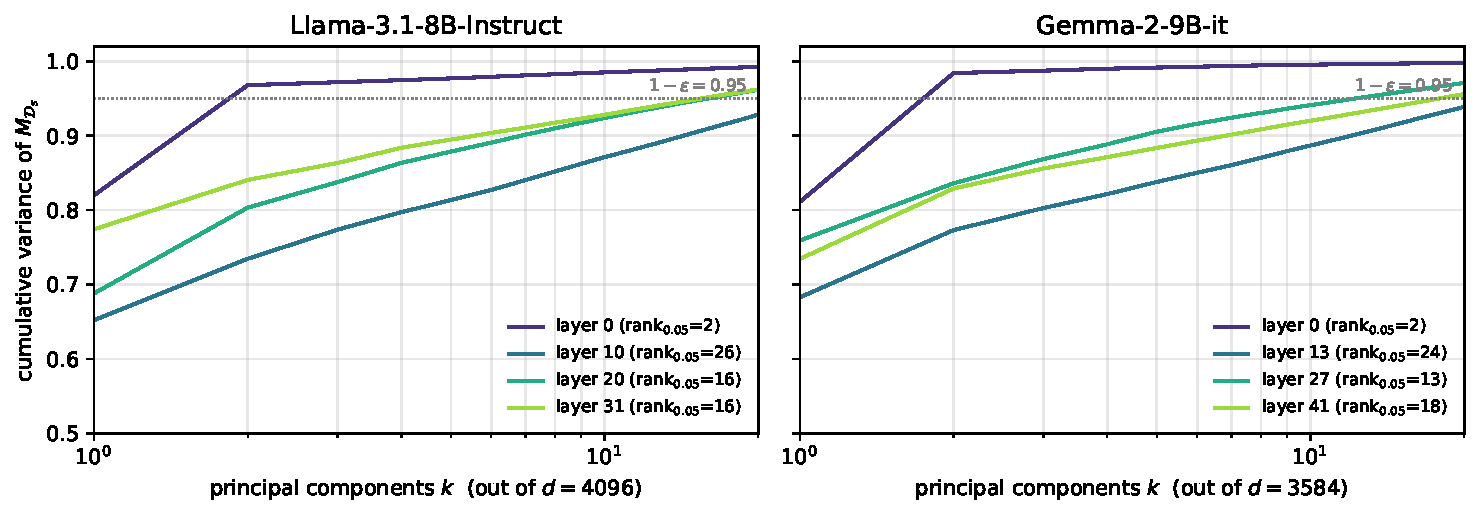
\includegraphics[width=\textwidth]{fig_diagnosis.pdf}
\caption{Per-layer cumulative variance of $M_{\mathcal{D}_s}$
for Llama and Gemma.  Fewer than $30$ components exceed
$1-\epsilon = 0.95$ against $d \geq 3584$.}
\label{fig:diagnosis}
\end{figure}

Fewer than $0.5\%$ of available directions account for
$95\%$ of variance.  By Definition~\ref{def:separable},
the modification is $(k, 0.05)$-separable with
$k=12,17,16$ for Llama/Gemma/Qwen.
$\rho_{\epsilon}(\mathcal{D}_s)$ is $\sim 50\%$ of
$\rho_{\epsilon}(\mathcal{D}_c)$: safety is more
concentrated than the general post-training shift.

\paragraph{Mean-direction decomposition.}
Subtracting the column mean
$\bar{m} := \frac{1}{n}\sum_i (h_{\mathrm{align}}(x_i) -
h_{\mathrm{pre}}(x_i))$ before SVD yields residual
effective rank $\sim 75$--$80$, $4$--$7\times$ the
uncentered value
(Table~\ref{tab:centered_vs_uncentered_body}).
A single mean-shift direction $\bar{m}\,\mathbf{1}^\top$
captures the bulk; its cosine with $u_1$ is $\sim 1$
by construction
(Table~\ref{tab:diagnosis_cos}).
On $M_{\mathrm{DiD}}$ (control-mean-subtracted), $u_1$
recovers the Arditi intra-aligned refusal direction at
$|\cos|\sim 0.77,0.86,0.50$ (Llama/Gemma/Qwen,
App.~\ref{app:arditi}); uncentered $M_{\mathcal{D}_s}$
gives only $\sim 0.34/0.39/0.18$ because it is
dominated by the chat-template shift
(Remark~\ref{rem:k1_arditi}).

\begin{table}[h]\centering
\caption{Centered vs.\ uncentered $\overline{\operatorname{rank}_{\epsilon}}$
on $M_{\mathcal{D}_s}$, mean across hidden layers.}
\label{tab:centered_vs_uncentered_body}
\begin{tabular}{@{}lcc@{}}
\toprule
Model & uncentered $\overline{\operatorname{rank}_{\epsilon}}$
      & centered $\overline{\operatorname{rank}_{\epsilon}}$ \\
\midrule
Llama-3.1-8B-Instruct & $12.0$ & $77.6$ \\
Gemma-2-9B-it         & $17.4$ & $76.2$ \\
Qwen-2.5-7B-Instruct  & $15.7$ & $80.4$ \\
\bottomrule
\end{tabular}
\end{table}

The uncentered rank is what the principal-subspace
ablation (\S\ref{sec:diagnosis_ablation}) targets and
what Proposition~\ref{prop:faking} controls.  The
framework does not claim a multi-dimensional safety
code: it formalizes the structural consequences of
the (known) single-direction structure.  The
calibration variants that change $\rho_{\epsilon}$ by
orders of magnitude (\S\ref{sec:calibration},
App.~\ref{app:calibration_v2}) operate by distributing
the mean direction across components.

The LRH baseline (App.~\ref{app:lrh}) gives
$\rho_{\epsilon} \approx 0.008$--$0.010$ on arbitrary
concepts, only $2$--$3\times$ the safety value: rank
alone is not a safety-specific signature.  The
safety-specific bridge is the causal ablation
(\S\ref{sec:diagnosis_ablation}), which collapses
refusal without breaking instruction-following on
$\mathcal{D}_c$.

\subsection{Principal direction alignment}

Table~\ref{tab:diagnosis_cos} reports
$|\cos(u_1, \bar{\Delta})|$ where $\bar{\Delta} =
\frac{1}{n}\sum_i (h_{\mathrm{align}}(x_i)
 - h_{\mathrm{pre}}(x_i))$.

\begin{table}[h]
\centering
\caption{Principal direction alignment:
$\overline{|\cos(u_1, \bar{\Delta})|}$ across layers.}
\label{tab:diagnosis_cos}
\begin{tabular}{@{}lc@{}}
\toprule
Model & Mean $|\cos\theta|$ \\
\midrule
Llama-3.1-8B-Instruct & $0.9996$ \\
Gemma-2-9B-it & $0.9993$ \\
\bottomrule
\end{tabular}
\end{table}

$u_1$ aligns with $\bar{\Delta}$ at $|\cos|>0.999$:
the modification is concentrated in a single dominant
direction (the $k=1$ case of
Remark~\ref{rem:recoverability}).

\subsection{Causal ablation}
\label{sec:diagnosis_ablation}

We project out the top-$k$ principal subspace of
$M_{\mathrm{template}}$ at five narrow-band and
eight wide-band layers, and measure refusal on
$n_{\mathrm{gen}}=100$ held-out prompts.
Table~\ref{tab:diagnosis_abl} reports the headline
narrow-band $k=3$ result for all three models; full
sweep in App.~\ref{app:abl_sweep}.

\begin{table}[h]
\centering
\caption{Causal ablation at narrow band $[0.45L, 0.70L]$,
$k=3$, $n_{\mathrm{gen}}=100$, Wilson 95\% CIs.}
\label{tab:diagnosis_abl}
\begin{tabular}{@{}lccc@{}}
\toprule
Model & Baseline & Principal rank-$3$
  & Random rank-$3$ \\
\midrule
Llama-3.1-8B-Instruct
  & $0.97$ & $0.80$ \;[$0.71, 0.87$] & $0.94 \pm 0.00$ \\
Gemma-2-9B-it
  & $0.99$ & $\mathbf{0.00}$ \;[$0.00, 0.04$] & $0.99 \pm 0.00$ \\
Qwen-2.5-7B-Instruct
  & $0.96$ & $0.54$ \;[$0.44, 0.63$] & $0.95$ \;[$0.89, 0.98$] \\
\bottomrule
\end{tabular}
\end{table}

The three models span the qualitative spectrum.
\textbf{Gemma} collapses cleanly: narrow-band $k=3$
alone drops refusal $0.99 \to \mathbf{0.00}$ (random
control $0.99$).  \textbf{Qwen} sits in the middle:
$0.96 \to 0.54$ at $k=3$ and progressively to
$0.01$ at $k\geq 20$ (App.~\ref{app:abl_sweep_qwen}),
monotone in $k$.  \textbf{Llama} is the outlier: the
same $k=3$ ablation drops refusal only to $0.80$
(random $0.94$), and the narrow-band curve is
\emph{non-monotonic} at $k=5$ (refusal $0.92$).
Per-direction ablation
(Table~\ref{tab:perdir_llama_body}) shows $u_1$ alone
drops refusal to $0.84$ but $u_2$ alone is null
despite ranking second by $\sigma$.  SVD orders by
variance, not causal authority; the Gemma--Qwen--Llama
ordering ranks how cleanly the SVD ordering and the
causal ordering agree.

\begin{table}[h]\centering
\caption{Per-direction narrow-band ablation,
Llama, baseline $0.97$.  Each row ablates a
\emph{single} direction (rank-$1$ projection out of the
named $u_i$ across the narrow-band layers); the
$u_3$--$u_5$ row reports the common refusal rate of
$0.94$ obtained for each of $u_3$, $u_4$, $u_5$
individually (per-direction values $0.94, 0.94, 0.94$).}
\label{tab:perdir_llama_body}
\begin{tabular}{@{}lcc@{}}
\toprule
Ablate & Refusal & Note \\
\midrule
$u_1$ alone & $0.84$ & strong refusal-promoting \\
$u_2$ alone & $0.99$ & near-zero causal effect \\
each of $u_3$--$u_5$ alone & $0.94$ & weak \\
\bottomrule
\end{tabular}
\end{table}

At wide band with $k=20$, Llama refusal collapses to
$\mathbf{0.00}$ (random $0.92$): the privileged
subspace is the same low-rank object, but in Llama it
is distributed across more layers than in Gemma,
consistent with \citep{arditi2024refusal, wollschlager2025}.

\paragraph{Mechanism reading of the $k=5$ non-monotonicity.}
The narrow-band Llama trajectory
$0.85 \to 0.80 \to \mathbf{0.92} \to 0.66 \to 0.10$
(at $k = 1,3,5,10,20$) cannot be read off the SVD
spectrum: tail singular values do not decrease
behavioral effect monotonically.  The per-direction
table decomposes the rebound: $u_1$ alone is
load-bearing (refusal $0.84$); $u_2$ alone is null;
$u_3$--$u_5$ are individually weak ($\sim 0.94$).  At
$k=3$ the ablation already covers the load-bearing
$u_1$ together with the inert $u_2$ and one of the
weak directions, dropping refusal to $0.80$.  At $k=5$ the rebound to $0.92$ is consistent with a
\emph{redundancy-with-interaction} reading: ablating
$u_1$ \emph{together} with $u_2,\ldots,u_5$ would
activate a compensatory pathway absent under $u_1$-only
or $u_1+\{u_2,u_3\}$ ablation, requiring $k\geq 10$ to
cover.  This reading is consistent with the concept-cone
refinement of \citet{wollschlager2025} and with the
wide-band $k=20$ result that collapses refusal to
$\mathbf{0.00}$, but the present per-direction data
alone does not distinguish it from alternatives (e.g.\
keyword-classifier interaction with specific token
distributions at $k=5$, or layer-interaction effects
across the narrow band); combination ablations on
non-consecutive subsets of the top-$k$ block, which we
do not run here, would be required to verify.  The
audit takeaway is robust to which reading is correct:
Test~2 must be evaluated as a curve in $k$ and the SVD
ordering is not a substitute for per-direction or
combination-aware ablation.

\subsection{Summary}

Principal rank-$k$ ablation collapses refusal to Wilson
$95\%$ CI $\subset [0.00, 0.05]$ in all three models
(Gemma at narrow $k=1$, Qwen at narrow $k\geq 20$,
Llama at wide $k=20$) while random rank-$k$ ablation
at the same layers leaves refusal intact.  The
diagnosed modification is therefore $(k,0.05)$-separable
with $k \leq 24$ against $d \geq 3584$, so
Propositions~\ref{prop:fragility} and~\ref{prop:faking}
apply.


% ============================================================================
\section{Discussion}
\label{sec:discussion}
% ============================================================================

\subsection{Scope: What the Diagnostic Measures}
\label{sec:discussion_what}

$\rho_{\epsilon}$ is a readout-level rank measurement
on a pre-defined safety distribution.
\textbf{(1) Low rank is generic, safety is at the
concentrated end.}  LRH baseline (App.~\ref{app:lrh}):
arbitrary concepts give $\rho_{\epsilon}\!\approx\!0.008$--$0.010$,
$2$--$3\times$ the safety value.  Test~2 supplies the
bridge from rank to behavior.
\textbf{(2) Readout, not mechanism}
(Remark~\ref{rem:readout_vs_mechanism}): a non-linear
computation writing into a low-dim subspace tests as
low-rank.  Fragility (Prop.~\ref{prop:fragility})
applies to residual-stream attacks; LoRA fine-tuning,
prompt jailbreaks, and deceptive alignment are out of
scope.
\textbf{(3) Headline rank is the Arditi mean direction
plus formatting variance} (\S\ref{sec:diagnosis_rank}): centered SVD
residual is $4$--$7\times$ uncentered.  Our contribution
is the index $\rho_{\epsilon}$ and the constructive
calibration, not a multi-dim safety code.

$\rho_{\epsilon}$ normalizes by nominal $d$ (intrinsic
dim is smaller, so reported numbers understate the
occupied fraction).  Rank-and-layer ablation does not
stratify by harm type; per-category structure is open.

\subsection{Where the Two-Stage Paradigm Discussion Sits}
\label{sec:discussion_paradigm}

It is tempting to argue that the two-stage paradigm
itself \emph{causes} low-rank alignment modifications:
that a narrow post-hoc objective on a frozen substrate
must produce a low-rank shift.  This argument is
plausible but exceeds our evidence.  Our measurements
show that three specific two-stage pipelines
(Llama-3.1, Gemma-2, Qwen-2.5 instruction tuning)
produce low-$\rho_{\epsilon}$ readouts; they do not
show that this is necessary, nor that single-stage
joint training would produce high-$\rho_{\epsilon}$
readouts.  A single-stage training run with
overwhelmingly more data devoted to general capability
than to safety might well produce the same readout
structure for the same data-imbalance reason.  We
therefore describe the two-stage observation as a
correlation: this is what current pipelines empirically
do, and it is sufficient to make the linear-projection
fragility of Prop.~\ref{prop:fragility} applicable.
Whether the readout is low-rank because of the paradigm
or because of the loss-imbalance asymmetry between
pre-training and alignment data is left open.

\subsection{Rank Inflation Does Not Buy Robustness}
\label{sec:discussion_position}

The same $\rho_{\epsilon} \approx 0.40$ can be either
ablation-robust ($\lambda=5$: $\geq 0.97$ through
$r=80$) or brittle ($\lambda=50$: $0.10$ at $r=40$;
App.~\ref{app:calibration_v2_ablation}).
$\rho_{\epsilon}$ screens for fragility but does not
certify that the high-rank shift is causally
distributed; Test~2 must be run separately.  The right
use is auditing existing alignments and flagging the
failure mode of Prop.~\ref{prop:fragility}; how to
train high-$\rho_{\epsilon}$ alignment at LLM scale is
open.

Diagnosed checkpoints are SFT/RLHF~\citep{ouyang2022}/DPO~\citep{rafailov2023dpo};
applying the diagnostic to Constitutional AI~\citep{bai2022},
debate~\citep{irving2018ai}, or IDA is an obvious next
step (see \S\ref{sec:discussion_paradigm} for what the
present measurements do and do not imply about the
two-stage paradigm in general).


% ============================================================================
\section{Open Problem: Faking-Footprint Lower Bound}
\label{sec:open}
% ============================================================================

Prop.~\ref{prop:faking} shows that a deceptive policy
\emph{can} mode-toggle with $O(\rho_{\epsilon}d)$
representational dimensions: the achievability direction
is unconditional.  The structural converse---any
successful faker \emph{must} use at least
$\Omega(\rho_{\epsilon}d)$ dimensions---is the
contrapositive ``high $\rho_{\epsilon}$ blocks low-cost
mode-toggling.''  We
sketch a Mirsky-based argument under a spectral-gap
hypothesis, show that the hypothesis is empirically
not satisfied across the unsafe-mode references we
tested, and identify a geometric reason
(Lemma~\ref{lem:kappa_obstruction}) that this proof
technique cannot be applied uniformly over the natural
$\epsilon$-budget faker class.  A matching
$\Omega(\rho_{\epsilon}d)$ lower bound by a different
route remains open.

\paragraph{Three quantities to distinguish.}
The argument involves three quantities the literature
conflates:
\begin{itemize}[nosep]
  \item $\kappa_{\mathrm{def}}(h^{(\cdot)}) :=
        \sigma_r(S)^2 / (\|E_1\|_F^2 + \|E_0\|_F^2)$:
        the per-mode-residual gap of a \emph{specific}
        faker, where $E_1 := M^{(1)} - M^{\mathrm{honest}}$
        (monitored-mode residual against the honest
        target) and
        $E_0 := M^{(0)} - M^{\mathrm{unsafe}}$
        (unmonitored-mode residual against the unsafe
        target).
  \item $\kappa_{\mathrm{lb}} :=
        \sigma_r(S)^2 / (\epsilon\,(\|M^{\mathrm{honest}}\|_F^2 +
        \|M^{\mathrm{unsafe}}\|_F^2))$:
        the worst-case lower bound on
        $\kappa_{\mathrm{def}}$ over the
        \emph{target-relative} $\epsilon$-budget class
        $\{\|E_1\|_F^2 \leq \epsilon\|M^{\mathrm{honest}}\|_F^2,
        \|E_0\|_F^2 \leq \epsilon\|M^{\mathrm{unsafe}}\|_F^2\}$
        (the faker-relative version
        $\|E_m\|_F^2 \leq \epsilon\|M^{(m)}\|_F^2$ differs
        by $\mathcal{O}(\sqrt{\epsilon})$ through
        $\|M^{(m)}\| \leq \|M^{\mathrm{target}}\| + \|E_m\|$
        and gives the same conclusion).
  \item $\kappa_{\mathrm{emp}}$: the empirical estimate
        of $\kappa_{\mathrm{lb}}$ (App.~\ref{app:kappa}).
\end{itemize}

\paragraph{Mirsky route, sketched.}
With $S := M^{\mathrm{honest}} - M^{\mathrm{unsafe}}$,
$r := \operatorname{rank}_{\epsilon}(S)$, and any
$\epsilon$-budget faker producing residuals $E_m$,
$\Delta M = S - E$ where $E := E_1 - E_0$.
Mirsky~\citep[][Thm.\ A.4]{stewart1990matrix} gives
$\sum_i (\sigma_i(\Delta M) - \sigma_i(S))^2 \leq
\|E\|_F^2 \leq 2(\|E_1\|_F^2 + \|E_0\|_F^2)$.
If $\sigma_r(S)^2 \geq \kappa_{\mathrm{def}}\,
(\|E_1\|_F^2 + \|E_0\|_F^2)$ holds with
$\kappa_{\mathrm{def}} > 8$, then
$\beta := \sqrt{2/\kappa_{\mathrm{def}}} < 1/2$ and
the perturbation $\|E\|_F \leq \beta\,\sigma_r(S)$
preserves $\sigma_i(\Delta M) \geq (1-\beta)\,\sigma_i(S)$
for $i \leq r$.  Combining this with the triangle bound
$\|\Delta M\|_F \leq \|S\|_F + \|E\|_F$, a tail-mass
argument on the perturbed top-$r$ block yields
$\operatorname{rank}_{\epsilon'}(\Delta M) \geq r$ for
some $\epsilon' > 0$ depending on $\beta$ and
$\epsilon$.  This is the matching $\Omega(r)$ lower
bound, \emph{provided} the threshold $\kappa > 8$
(equivalently $\beta < 1/2$) holds uniformly over the
$\epsilon$-budget faker class.  The next lemma shows
this uniform provision cannot be supplied.

\begin{lemma}[Spectral-gap budget bound]
\label{lem:kappa_obstruction}
For any honest/unsafe pair $(M^h, M^u)$ with
$S = M^h - M^u$ and $r = \operatorname{rank}_{\epsilon}(S)$,
\begin{equation}
  \kappa_{\mathrm{lb}}
   = \frac{\sigma_r(S)^2}
          {\epsilon\,(\|M^h\|_F^2 + \|M^u\|_F^2)}
   \;\leq\; \frac{2}{\epsilon\,r}.
  \label{eq:kappa_obstruction}
\end{equation}
\end{lemma}

\begin{proof}
$\sigma_r(S)$ is the smallest of the top-$r$ singular
values, so $\sigma_r(S)^2 \leq \frac{1}{r}\sum_{i=1}^{r}
\sigma_i(S)^2 \leq \|S\|_F^2/r$.  Triangle inequality
applied entrywise gives $\|S\|_F^2 = \|M^h - M^u\|_F^2
\leq 2(\|M^h\|_F^2 + \|M^u\|_F^2)$.  Combining,
$\sigma_r(S)^2 \leq (2/r)(\|M^h\|_F^2 + \|M^u\|_F^2)$;
divide both sides by $\epsilon(\|M^h\|_F^2 +
\|M^u\|_F^2)$.
\end{proof}

\begin{corollary}[Mirsky route, uniformly unavailable]
\label{cor:mirsky_obstruction}
$\kappa_{\mathrm{lb}} \leq 8$ whenever $\epsilon r \geq
1/4$, and $\kappa_{\mathrm{lb}} < 8$ whenever
$\epsilon r > 1/4$.  At $\epsilon = 0.05$, this means
$r \geq 5$ already gives $\kappa_{\mathrm{lb}} \leq 8$,
and $r \geq 6$ gives strict $\kappa_{\mathrm{lb}} < 8$.
The Mirsky-route sketch, which requires the strict
threshold $\kappa > 8$ uniformly over the
$\epsilon$-budget faker class, therefore cannot deliver
the matching $\Omega(r)$ lower bound whenever $S$ has
$\operatorname{rank}_{\epsilon}(S) \geq 6$
($\epsilon = 0.05$).
\end{corollary}

\paragraph{Scope of the open problem.}
Lemma~\ref{lem:kappa_obstruction} is a
\emph{proof-technique} statement about the present
Mirsky route, not a refutation of the structural
converse.  \textbf{What is closed:} the Mirsky route to
a matching $\Omega(\rho_{\epsilon}d)$ lower bound
\emph{uniformly} over the $\epsilon$-budget faker class
$\{\|E_1\|_F^2 \leq \epsilon\|M^{\mathrm{honest}}\|_F^2,
\|E_0\|_F^2 \leq \epsilon\|M^{\mathrm{unsafe}}\|_F^2\}$,
since the spectral-gap hypothesis $\kappa > 8$ required
by the sketched argument is incompatible with
$\kappa_{\mathrm{lb}} \leq 2/(\epsilon r)$ once
$\epsilon r > 1/4$.  \textbf{What remains open:}
tighter faker classes with $\|E_m\|_F^2 \ll
\epsilon\|M^{\mathrm{target}}\|_F^2$ may give
$\kappa_{\mathrm{def}} > 8$ for specific deceptive
policies (the obstruction binds only the worst-case
$\kappa_{\mathrm{lb}}$), and non-Mirsky routes---e.g.\
Davis--Kahan principal-angle bounds or
causal-subspace substitutes for the SVD subspace---are
not addressed.  The empirical results below ($1/90$,
$0/36$) thus confirm the obstruction binds in practice,
not that the structural converse itself is false.

\paragraph{Empirical status: the spectral gap fails
across the unsafe references we tested.}
On three Llama-3.1-8B-Instruct unsafe references
(distinct uncensoring techniques, App.~\ref{app:kappa}),
$\kappa_{\mathrm{emp}} > 8$ on $1/90$ layer-reference
pairs (mlabonne L$0$, where $S$ degenerates to rank-$1$
because the input-adjacent layer is dominated by a
single mean shift induced by the abliteration weight
edit before the residual stream has integrated
context-dependent structure).
Median $\kappa_{\mathrm{emp}} = 0.007$.  In the
calibration MLP across $4$ honest$\times$unsafe
pairings (App.~\ref{app:calibration_kappa}), $0/36$
combinations cross $\kappa = 8$; the maximum is $2.64$
in the most concentrated pair, and the
distributed--vs--distributed pair gives the worst case
($\max = 0.07$): broadening the unsafe shift raises
the denominator faster than $\sigma_r(S)^2$.  The
spectral-gap hypothesis is hardest to satisfy precisely
in the distributed-alignment regime that high
$\rho_{\epsilon}$ targets.

\paragraph{Two open questions.}
(1) Is there an unsafe-mode construction (e.g.\ a
deliberately fine-tuned harmful variant trained to span
a different subspace from the honest alignment, not
just remove the refusal direction) for which
$\kappa_{\mathrm{emp}} > 8$ holds on a non-trivial
fraction of layers?  (2) Is there a different
lower-bound argument that does not require a
spectral-gap hypothesis and delivers
$\Omega(\rho_{\epsilon}d)$ for a more permissive class
of deceptive policies?  Both remain genuinely open;
the present work establishes only the achievability
side (Prop.~\ref{prop:faking}) and the obstruction to
the natural Mirsky-route converse
(Lemma~\ref{lem:kappa_obstruction}).


% ============================================================================
\section{Related Work}
\label{sec:related}
% ============================================================================

\paragraph{Empirical fragility.}
Safety fine-tuning is empirically
fragile~\citep{qi2023finetuning, lermen2023lora,
qi2024safety, betley2025emergent},
and models elastically resist alignment as a
shallow overlay~\citep{ji2025elasticity}.
The rank diagnostic groups these phenomena under a
common geometric prerequisite: low
$\rho_{\epsilon}$ at the relevant residual layers
makes them all available.

\paragraph{Mechanistic interpretability.}
\citet{arditi2024refusal} introduced the intra-aligned
refusal direction $\bar{\Delta}^{\mathrm{Arditi}} =
\mathbb{E}_{\mathcal{D}_s}[h_{\mathrm{align}}] -
\mathbb{E}_{\mathcal{D}_c}[h_{\mathrm{align}}]$,
computed on the aligned model alone, and showed
ablating it removes refusal.  Our $M_{\mathcal{D}_s}$
is a different object: the paired alignment-stage shift
$h_{\mathrm{align}} - h_{\mathrm{pre}}$, which requires
both checkpoints and conflates alignment-induced
structure with chat-template formatting structure
($M_{\mathrm{template}}$ controls for the chat-template
confound at the collection level, $M_{\mathrm{DiD}}$
further removes the cross-prompt template-asymmetry
component and recovers the Arditi direction with
$|\cos|$ up to $0.86$).
\citet{wollschlager2025} showed refusal is mediated by
concept \emph{cones}---multiple causally relevant
directions, not a single one---and our centered-SVD
residual rank $\sim 75$--$80$ on $M_{\mathcal{D}_s}$ is
consistent with this multi-dimensional picture rather
than independent of it: we re-measure the
multi-dimensional structure under the four-variant
control, but the existence of multi-dimensional
structure beyond the rank-$1$ direction is established
by \citet{wollschlager2025}.
\citet{jain2024what, lee2024mechanistic} provide
mechanistic accounts of safety fine-tuning and
DPO~\citep{rafailov2023dpo}.
Representation engineering~\citep{zou2023representation,
turner2023steering} demonstrates the operational
side of what $\rho_{\epsilon}$ measures: a
distinguishable low-rank subspace can be steered or
removed.  Sparse-autoencoder
work~\citep{templeton2024scaling} provides an
alternative decomposition basis with monosemantic
features; whether SAE-recovered features give a more
causally aligned rank than SVD components on
$M_{\mathcal{D}_s}$ is a natural open question (we use
SVD because it is sub-capable computable from paired
checkpoints alone).
Our contribution is the formal index, the
chat-template-controlled four-variant decomposition,
and the Mirsky-route scoping
(Lemma~\ref{lem:kappa_obstruction}); mechanism-level
discovery is not claimed.

\paragraph{Deceptive alignment.}
\citet{greenblatt2024alignment, hubinger2024sleeper}
demonstrate alignment faking and its persistence.
Proposition~\ref{prop:faking} formalizes the
\emph{representational footprint} of mode-toggling
($O(\rho_{\epsilon} d)$ achievability);
the value-misalignment-driven adversarial pressure
that produces deception is outside our scope.

\paragraph{Scalable oversight and theory.}
\citet{burns2023weak, leike2018scalable,
amodei2016concrete, irving2018ai} seek scalable
oversight; \citet{wolf2024fundamental} proves
information-theoretic alignment limits;
\citet{ngo2024alignment} surveys the field.
The sub-capable computability of $\rho_{\epsilon}$
(Remark~\ref{rem:bootstrap}) provides a
complementary structural-measurement primitive.

\paragraph{Linear representations.}
LLMs encode many concepts
linearly~\citep{mikolov2013linguistic,
park2024linear, marks2023geometry, hernandez2024linearity};
sparse autoencoders~\citep{templeton2024scaling}
decompose this further.
Low $\rho_{\epsilon}$ on $M_{\mathcal{D}_s}$ is
consistent with this null;
Test~2 (causal ablation) measures the additional
content beyond linearity, namely whether the
low-rank subspace is causally privileged.

\paragraph{LoRA, concept erasure, mode connectivity.}
\citet{hu2022lora}'s low-rank adaptation is
weight-space; our activation-space low-rank
structure is consistent but not entailed.
Concept erasure~\citep{ravfogel2020null,
belrose2023leace} provides upper bounds on
linear-projection ablation;
mode-connectivity~\citep{garipov2018loss,
frankle2020linear} explains why small parameter
perturbations~\citep{lermen2023lora} can undo
alignment.

\bibliography{references}
\bibliographystyle{tmlr}


\appendix

% ============================================================================
\section{Extended Diagnostic Results}
\label{app:rank_sweep}
% ============================================================================

Extended diagnostic results referenced in
Sections~\ref{sec:diagnosis_setup}--\ref{sec:diagnosis_ablation}.
Full numerics in \verb|experiments/v4/results/|.

\subsection{Four modification-matrix variants}
\label{app:four_variants}

\begin{table}[h]\centering
\caption{Four modification-matrix variants on Llama-3.1-8B-Instruct,
$\rho_{\epsilon}$ on $\mathcal{D}_s$, mean across hidden layers,
$n = 200$.  $M_{\mathrm{template}}$ controls for the
chat-template confound (both checkpoints evaluated under
the same template); $M_{\mathrm{naive}}$ leaves it
uncontrolled; $M_{\mathrm{DiD}}$ further subtracts the
$\mathcal{D}_c$ column-mean to remove the cross-prompt
component of the residual template asymmetry,
recovering the Arditi direction at higher cosine.}
\label{tab:four_variants_llama}
\begin{tabular}{@{}lc@{}}
\toprule
Variant & $\overline{\rho_{\epsilon}}(\mathcal{D}_s)$ \\
\midrule
$M_{\mathrm{naive}}$ (v3 quantity) & $0.0113$ \\
$M_{\mathrm{template}}$ (chat-template controlled)
  & $0.0029$ \\
$M_{\mathrm{aligned}}$ (alignment-stage shift only)
  & $0.0133$ \\
$M_{\mathrm{DiD}}$ (control-subtracted) & $0.0101$ \\
\bottomrule
\end{tabular}
\end{table}

\subsection{Bootstrap stability of $\operatorname{rank}_{\epsilon}$ across three LLM families}
\label{app:bootstrap}

We bootstrap-resample the $n=200$ paired
safety-relevant samples with replacement ($200$
resamples per layer) and recompute
$\operatorname{rank}_{\epsilon}$ on
$M_{\mathrm{template}}$ at $\epsilon = 0.05$.  The
resampling distribution is tight ($\pm 1$ to $\pm 2$
across all layers and all three families) and centered
\emph{below} the full-sample (without-replacement)
point estimate, with the gap growing with rank---this
is the standard downward bias of with-replacement
bootstrap on rank functionals (resampling reduces the
effective unique sample size to ${\approx}0.63n$,
shrinking the recovered rank).  The bootstrap remains
useful as a stability check on relative variability;
the full-sample column is the rank reported in
Table~\ref{tab:diagnosis_rank} and
Table~\ref{tab:n_sweep}.

\begin{table}[h]\centering
\caption{Bootstrap-resample distribution
(with replacement, $n_{\mathrm{boot}}=200$) of
$\operatorname{rank}_{\epsilon}(M_{\mathrm{template}})$
at $\epsilon=0.05$, alongside the full-sample
(without-replacement) point estimate at $n=200$.  The
bootstrap mean is systematically below the full-sample
rank by ${\approx}1$--$13$ depending on rank
magnitude---an artifact of with-replacement resampling
on a non-smooth functional, not a CI for the underlying
rank.}
\label{tab:bootstrap_ci}
\begin{tabular}{@{}llccccc@{}}
\toprule
Family & Layer & Full-sample & Boot.\ mean & Boot.\ std
       & Boot.\ 95\% range \\
\midrule
Llama (L=32) & 14 & $19$ & $15.42$ & $0.66$ & $[14, 17]$ \\
             & 15 & $19$ & $15.59$ & $0.64$ & $[15, 17]$ \\
             & 16 & $17$ & $14.51$ & $0.62$ & $[13, 16]$ \\
             & 17 & $14$ & $11.95$ & $0.62$ & $[11, 13]$ \\
             & 18 & $13$ & $11.47$ & $0.58$ & $[11, 12]$ \\
\midrule
Gemma (L=42) & 19 & $27$ & $21.68$ & $0.92$ & $[20, 23]$ \\
             & 20 & $27$ & $21.68$ & $0.88$ & $[20, 23]$ \\
             & 21 & $24$ & $19.40$ & $0.87$ & $[18, 21]$ \\
             & 22 & $24$ & $19.66$ & $0.83$ & $[18, 21]$ \\
             & 23 & $23$ & $18.56$ & $0.82$ & $[17, 20]$ \\
\midrule
Qwen (L=28)  & 13 & $~5$ & $~5.04$ & $0.23$ & $[5,~6]$ \\
             & 15 & $~8$ & $~7.07$ & $0.33$ & $[7,~8]$ \\
             & 18 & $19$ & $15.67$ & $0.61$ & $[15, 17]$ \\
             & 21 & $33$ & $25.38$ & $0.87$ & $[24, 27]$ \\
             & 24 & $49$ & $35.91$ & $1.22$ & $[34, 38]$ \\
\bottomrule
\end{tabular}\\
\small Sources: \texttt{v4\_llama.json},
\texttt{v4\_gemma.json},
\texttt{revision6\_qwen\_bootstrap.json}.
\end{table}


\subsection{$\epsilon$-sensitivity of $\rho_{\epsilon}$}
\label{app:eps_sensitivity}

The headline $\rho_{\epsilon}$ in
\S\ref{sec:diagnosis_rank} uses $\epsilon=0.05$
(retain $95\%$ of variance).  Table~\ref{tab:eps_sens}
reports the narrow-band mean effective rank at three
$\epsilon$ values to show how the index moves with the
variance-tolerance choice.  The rank decreases
monotonically with $\epsilon$ across all three models;
at $\epsilon=0.20$ all three models collapse to
rank-$1$ (the Arditi mean direction).  Across the
$0.05$--$0.20$ range, $\rho_{\epsilon}$ moves by under
an order of magnitude.

\begin{table}[h]\centering
\caption{$\epsilon$-sensitivity of $\rho_{\epsilon}$ on
$M_{\mathrm{template}}$, mean over narrow-band Test~2
layers per family.  Computed from the stored
$M_{\mathrm{template}}$ top-$30$ singular values, with
total variance back-calculated from the stored
$\operatorname{rank}_{0.05}$ field.}
\label{tab:eps_sens}
\begin{tabular}{@{}lcccc@{}}
\toprule
Family & narrow band & $\epsilon=0.05$
  & $\epsilon=0.10$ & $\epsilon=0.20$ \\
\midrule
Llama  & layers $14,15,17,19,22$
  & $14.6/0.0036$ & $4.4/0.0011$ & $1.0/0.0002$ \\
Gemma  & layers $19,22,25,27,29$
  & $20.2/0.0056$ & $6.4/0.0018$ & $1.0/0.0003$ \\
Qwen   & layers $12,13,15,17,19$
  & $11.4/0.0032$ & $3.8/0.0011$ & $1.2/0.0003$ \\
\bottomrule
\end{tabular}\\
\small Each cell reports $\overline{\operatorname{rank}_{\epsilon}}/\rho_{\epsilon}$.
The $\epsilon=0.01$ regime requires more than the
stored $30$ singular values per layer and is omitted;
the corresponding entry would be $\geq 0.0073$
(Llama), $\geq 0.0084$ (Gemma), $\geq 0.0083$ (Qwen).
\end{table}


\subsection{Sample-size sweep}
\label{app:n_sweep}

To rule out a finite-sample artifact of the bound
$\operatorname{rank}_{\epsilon}\leq \min(d,n)$, we
sweep $n \in \{50, 100, 200\}$ on
$M_{\mathrm{template}}$ at a representative middle
layer.  Effective rank saturates well below $\min(d,n)$:
the rank is signal-driven, not sample-bound.

\begin{table}[h]\centering
\caption{Sample-size sweep at a representative middle
layer ($L=16$ for Llama, $L=21$ for Gemma; selected as
the median of the layer index range), $\epsilon=0.05$.
$\operatorname{rank}_{\epsilon}/\min(d,n)$ stays
$<\!0.25$ at $n{=}200$ for both models.}
\label{tab:n_sweep}
\begin{tabular}{@{}lccc@{}}
\toprule
Model, $n$ &
$\operatorname{rank}_{\epsilon}$ &
$\rho_{\epsilon}$ &
$\operatorname{rank}_{\epsilon}/\min(d,n)$ \\
\midrule
Llama, $n{=}50$  & $9$  & $0.0022$ & $0.180$ \\
Llama, $n{=}100$ & $16$ & $0.0039$ & $0.160$ \\
Llama, $n{=}200$ & $17$ & $0.0042$ & $0.085$ \\
\midrule
Gemma, $n{=}50$  & $12$ & $0.0033$ & $0.240$ \\
Gemma, $n{=}100$ & $22$ & $0.0061$ & $0.220$ \\
Gemma, $n{=}200$ & $24$ & $0.0067$ & $0.120$ \\
\bottomrule
\end{tabular}
\end{table}

\subsection{Rank-and-layer ablation sweep}
\label{app:abl_sweep}

Test~2 extended to $k \in \{1,3,5,10,20,50\}$ on Llama
narrow band $[0.45L, 0.70L]$, $n_{\mathrm{gen}} = 100$.
The wide band $[0.30L, 0.85L]$ gives a monotonic
collapse to $\mathbf{0.00}$ at $k \geq 20$; the
narrow-band non-monotonicity at $k=5$ is decomposed in
the body (Table~\ref{tab:perdir_llama_body}).

\begin{table}[h]\centering
\caption{Llama narrow-band ablation, refusal rate
(Wilson 95\% CI), $n_{\mathrm{gen}}=100$, baseline $0.97$.}
\label{tab:ablation_llama}
\begin{tabular}{@{}lccc@{}}
\toprule
$k$ & Principal & 95\% CI & Random \\
\midrule
1  & 0.85 & [0.77, 0.91] & 0.97 \\
3  & 0.80 & [0.71, 0.87] & 0.94 \\
5  & 0.92 & [0.85, 0.96] & 0.93 \\
10 & 0.66 & [0.56, 0.75] & 0.96 \\
20 & 0.10 & [0.06, 0.17] & 0.87 \\
50 & 0.03 & [0.01, 0.08] & 0.95 \\
\bottomrule
\end{tabular}
\end{table}

\paragraph{$M_{\mathrm{DiD}}$ ablation.}
$M_{\mathrm{DiD}}$ recovers the Arditi direction at
$|\cos|\sim 0.77$ vs.\ $0.34$ on $M_{\mathrm{template}}$
(\S\ref{sec:diagnosis_rank}).  At low rank
$k\in\{3,5,10\}$, $M_{\mathrm{DiD}}$ ablation produces
stronger refusal collapse; at $k\geq 20$,
$M_{\mathrm{template}}$ catches up because its
higher-rank projection sweeps in chat-template directions
absent from $M_{\mathrm{DiD}}$.

\begin{table}[h]\centering
\caption{Llama narrow-band $M_{\mathrm{DiD}}$ ablation,
$n_{\mathrm{gen}} = 100$, baseline $0.97$.}
\label{tab:ablation_llama_mdid}
\begin{tabular}{@{}cccc@{}}
\toprule
$k$ & $M_{\mathrm{DiD}}$ refusal & 95\% CI &
$M_{\mathrm{template}}$ ref. \\
\midrule
$1$  & $0.87$ & $[0.79, 0.92]$ & $0.85$ \\
$3$  & $\mathbf{0.69}$ & $[0.59, 0.77]$ & $0.80$ \\
$5$  & $\mathbf{0.79}$ & $[0.70, 0.86]$ & $0.92$ \\
$10$ & $\mathbf{0.50}$ & $[0.40, 0.60]$ & $0.66$ \\
$20$ & $0.27$ & $[0.19, 0.36]$ & $0.10$ \\
$50$ & $0.01$ & $[0.00, 0.05]$ & $0.03$ \\
\bottomrule
\end{tabular}
\end{table}

For Gemma-2-9B-it, narrow-band $k=1$ already collapses
refusal to $\mathbf{0.00}$ (random control $0.99$),
consistent with its more concentrated single-direction
structure.  $M_{\mathrm{DiD}}$ ablation was run only on
Llama; whether the low-$k$ advantage of
$M_{\mathrm{DiD}}$ over $M_{\mathrm{template}}$ holds on
Gemma and Qwen (where the Arditi cosine reaches $0.86$
and $0.50$ respectively) is open.  The headline Test~2
table (\S\ref{sec:diagnosis_ablation}) uses
$M_{\mathrm{template}}$ across all three families for a
uniform protocol; the $M_{\mathrm{DiD}}$ comparison
here is an additional Llama-only check that
chat-template-controlled and Arditi-recovering
quantities yield consistent qualitative conclusions at
low $k$.

\paragraph{Qwen narrow-band sweep.}
\label{app:abl_sweep_qwen}
On Qwen-2.5-7B-Instruct, the narrow-band trajectory is
monotone and progressive: refusal drops smoothly with
$k$ until saturation by $k\!\geq\!10$.

\begin{table}[h]\centering
\caption{Qwen narrow-band $M_{\mathrm{template}}$
ablation, $n_{\mathrm{gen}}=100$, baseline $0.96$.}
\label{tab:ablation_qwen}
\begin{tabular}{@{}lcc@{}}
\toprule
$k$ & Principal refusal & 95\% CI \\
\midrule
$1$  & $0.92$ & $[0.85, 0.96]$ \\
$3$  & $0.54$ & $[0.44, 0.63]$ \\
$5$  & $0.24$ & $[0.17, 0.33]$ \\
$10$ & $0.06$ & $[0.03, 0.12]$ \\
$20$ & $\mathbf{0.01}$ & $[0.00, 0.05]$ \\
$50$ & $\mathbf{0.01}$ & $[0.00, 0.05]$ \\
\bottomrule
\end{tabular}
\end{table}

Qwen's monotone collapse contrasts with Llama's $k=5$
non-monotonicity: the SVD ordering is closer to the
causal ordering in Qwen, but Qwen requires more
directions ($k\sim 10$) than Gemma ($k=1$) for full
collapse.

\subsection{Arditi refusal-direction comparison}
\label{app:arditi}

Absolute cosine similarity between Arditi's
intra-aligned refusal direction
$\bar{\Delta}^{\mathrm{Arditi}}$ and the top-$1$ left
singular vector of each variant.  The
DiD-corrected matrix recovers the Arditi direction at
high cosine.

\begin{table}[h]\centering
\caption{Mean-over-layers $|\cos|$ between
$\bar{\Delta}^{\mathrm{Arditi}} =
\mathbb{E}_{\mathcal{D}_s}[h_{\mathrm{align}}] -
\mathbb{E}_{\mathcal{D}_c}[h_{\mathrm{align}}]$ and
the top-$1$ singular vector of each variant.}
\label{tab:arditi_cos}
\begin{tabular}{@{}lccc@{}}
\toprule
Model & vs $M_{\mathrm{naive}}$
      & vs $M_{\mathrm{template}}$
      & vs $M_{\mathrm{DiD}}$ \\
\midrule
Llama-3.1-8B-Instruct & $0.319$ & $0.337$ & $\mathbf{0.772}$ \\
Gemma-2-9B-it         & $0.367$ & $0.388$ & $\mathbf{0.860}$ \\
Qwen-2.5-7B-Instruct  & ---     & $0.179$ & $\mathbf{0.504}$ \\
\bottomrule
\end{tabular}
\end{table}

Qwen $M_{\mathrm{DiD}}$ recovers Arditi at $|\cos| = 0.504$
mean (max $0.803$), lower than Llama/Gemma:
consistent with a more distributed safety mechanism, and
a reminder that the rank-$1$ collapse of \citet{arditi2024refusal}
is not universal.

\subsection{Linear-representation-hypothesis baseline}
\label{app:lrh}

$\rho_{\epsilon}$ on English-vs-French and
question-vs-statement concept-difference matrices,
compared to safety: low-rank concentration is more
pronounced for alignment than for generic linearly
represented concepts.

\begin{table}[h]\centering
\caption{LRH baseline: $\rho_{\epsilon}$ on
$M_{\mathrm{template}}$ vs.\ control concepts.}
\label{tab:lrh_baseline}
\begin{tabular}{@{}lcccc@{}}
\toprule
Model & EN-FR & Q-Stmt & Safety & ratio \\
\midrule
Llama-3.1-8B & $0.0078$--$0.0086$ & $0.0086$ & $0.0029$ & $2.7\times$ \\
Gemma-2-9B   & $0.0086$--$0.0104$ & $0.0090$ & $0.0048$ & $1.9\times$ \\
\bottomrule
\end{tabular}
\end{table}

\subsection{Calibration v2: constructive calibration}
\label{app:calibration_v2}

A Distributed variant trained with a stable-rank
surrogate plus column-orthogonality penalty verifies
the diagnostic across the spectrum.

\begin{table}[h]\centering
\caption{Calibration v2: aggregate $\rho_{\epsilon}$ on
$\mathcal{D}_s$, $3$--$5$ seeds.
$\lambda{=}5$ Distributed is the sweet spot;
$\lambda{=}50$ saturates $\rho_{\epsilon}$ but degrades
compliance (App.~\ref{app:calibration_v2_ablation}).}
\label{tab:calibration_v2}
\begin{tabular}{@{}lcc@{}}
\toprule
Variant & $\rho_{\epsilon}$ & Compliance \\
\midrule
Steering (rank-$1$)            & $0.008$ & $\geq 0.93$ \\
Full-fine-tune ($\lambda{=}0$) & $0.173$ & $\geq 0.93$ \\
Distributed ($\lambda{=}0.5$)  & $0.332$ & $0.94$ \\
Distributed ($\lambda{=}5$, sweet spot) & $\mathbf{0.400}$ & $\mathbf{0.86}$ \\
Distributed ($\lambda{=}50$, brittle)   & $0.405$ & $0.71$ \\
\bottomrule
\end{tabular}
\end{table}

\subsection{Calibration v2: Test~2 projection ablation per variant}
\label{app:calibration_v2_ablation}

Test~2 ablation (\S\ref{sec:diagnosis_ablation}) applied
to FullFT and Distributed at $\lambda \in \{0.5, 5,
15, 50\}$.  Tests the contrapositive of
Prop.~\ref{prop:fragility}: high-$\rho_{\epsilon}$
alignments should resist low-rank projection.
(Independent of the Mirsky converse;
see~\S\ref{sec:open}.)

\begin{table}[h]\centering
\caption{Post-ablation compliance on $\mathcal{D}_s$,
final hidden layer ($d=128$), $3$ seeds.}
\label{tab:calibration_v2_ablation}
\begin{tabular}{@{}lcccccccc@{}}
\toprule
Variant & $\rho_{\epsilon}$
        & $r{=}0$ & $r{=}1$ & $r{=}3$ & $r{=}10$
        & $r{=}20$ & $r{=}40$ & $r{=}80$ \\
\midrule
FullFT ($\lambda{=}0$)        & $0.175$ & $0.96$ & $1.00$ & $0.84$ & $0.68$ & $0.76$ & $0.26$ & $0.07$ \\
Distributed ($\lambda{=}0.5$) & $0.332$ & $0.94$ & $0.97$ & $0.97$ & $1.00$ & $0.97$ & $1.00$ & $1.00$ \\
Distributed ($\lambda{=}5$)   & $0.400$ & $0.86$ & $0.90$ & $0.93$ & $1.00$ & $1.00$ & $1.00$ & $1.00$ \\
Distributed ($\lambda{=}15$)  & $0.404$ & $0.78$ & $0.78$ & $0.84$ & $0.88$ & $1.00$ & $1.00$ & $0.68$ \\
Distributed ($\lambda{=}50$)  & $0.405$ & $0.71$ & $0.78$ & $0.87$ & $0.93$ & $0.34$ & $0.10$ & $0.14$ \\
\bottomrule
\end{tabular}
\end{table}

FullFT ($\rho_{\epsilon}\!\approx\!0.175$) collapses to
$0.07$ at $r{=}80$; Distributed
$\lambda\in\{0.5,5\}$ holds $\geq 0.97$ through $r{=}80$.
The trade-off is non-monotone: at $\lambda \geq 15$,
$\rho_{\epsilon}$ stays $\sim 0.40$ but compliance
collapses---rank inflation without preserving the
safety signal.  High $\rho_{\epsilon}$ \emph{can} be
ablation-robust, but not every training that raises
$\rho_{\epsilon}$ does, which is the precise sense in
which $\rho_{\epsilon}$ is necessary but not sufficient.

\subsection{Empirical spectral-gap measurement across three unsafe-mode references}
\label{app:kappa}

The Mirsky-route hypothesis (\S\ref{sec:open}) requires
$\kappa > 8$ on $S = M^{\mathrm{honest}} - M^{\mathrm{unsafe}}$.
We measure $\kappa_{\mathrm{emp}}(\ell) :=
\sigma_r(S_\ell)^2 / (\epsilon\,(\|M^h_\ell\|_F^2
+ \|M^u_\ell\|_F^2))$ on three Llama-3.1-8B-Instruct
unsafe-mode references (\texttt{mlabonne abliterated},
\texttt{Lexi-Uncensored-V2}, \texttt{DarkIdol-Uncensored}),
$r = \operatorname{rank}_{0.05}(S_\ell)$, $n=200$.

\begin{table}[h]\centering
\caption{Per-reference $\kappa_{\mathrm{emp}}$ on Llama
($n=200$). $1/90$ layer-reference pairs cross $\kappa=8$
(mlabonne L$0$, an input-adjacent rank-$1$ degenerate case).}
\label{tab:kappa_emp}
\begin{tabular}{@{}lcccc@{}}
\toprule
Reference & layers & $\kappa>8$ & median & max \\
\midrule
mlabonne abliterated     & $32$ & $1$ & $0.007$ & $8.64$ \\
Lexi-Uncensored-V2       & $26$ & $0$ & $0.005$ & $0.006$ \\
DarkIdol Uncensored 1.2  & $32$ & $0$ & $0.009$ & $0.087$ \\
\midrule
\textbf{Aggregate}       & $\mathbf{90}$ & $\mathbf{1}$ & $\mathbf{0.007}$ & $\mathbf{8.64}$ \\
\bottomrule
\end{tabular}
\end{table}

No middle or late layer crosses for any reference:
across three uncensoring techniques, modal-difference
tail singular values are comparable to the per-mode
noise budget at $\epsilon=0.05$.  \S\ref{sec:open}
accordingly states the lower bound as open.

\subsection{Calibration MLP $\kappa_{\mathrm{emp}}$ across honest/unsafe regularization regimes}
\label{app:calibration_kappa}

To check whether the LLM negative
(App.~\ref{app:kappa}) is artifact or structural, we
sweep the four honest$\times$unsafe pairings in the
calibration MLP: \texttt{ft} ($\rho_{\epsilon}\!\approx\!0.17$),
\texttt{dist5} ($\rho_{\epsilon}\!\approx\!0.40$),
\texttt{unsafe\_ft}, \texttt{unsafe\_dist5}; $3$ seeds,
$3$ layers, $d = 128$.

\begin{table}[h]\centering
\caption{Calibration MLP $\kappa_{\mathrm{emp}}$ across
$9$ seed--layer pairs per pairing.  Zero pairings
cross $\kappa = 8$.  Counter-intuitively, the largest
$\kappa$ comes from \texttt{ft} vs.\ \texttt{unsafe\_ft}
($\max = 2.64$); broadening modal shift raises the
per-mode noise budget faster than it raises
$\sigma_r(S)$.}
\label{tab:calibration_kappa}
\begin{tabular}{@{}lcccc@{}}
\toprule
honest \& unsafe pairing & $r_S$ median &
$\kappa$ median & $\kappa$ max & layers $\kappa>8$ \\
\midrule
\texttt{ft}     vs.\ \texttt{unsafe\_ft}     & $11$ & $0.090$ & $\mathbf{2.64}$ & $0/9$ \\
\texttt{ft}     vs.\ \texttt{unsafe\_dist5}  & $24$ & $0.047$ & $0.19$ & $0/9$ \\
\texttt{dist5}  vs.\ \texttt{unsafe\_ft}     & $66$ & $0.051$ & $0.09$ & $0/9$ \\
\texttt{dist5}  vs.\ \texttt{unsafe\_dist5}  & $61$ & $0.046$ & $0.07$ & $0/9$ \\
\midrule
\textbf{Aggregate}                            & --- & $0.058$ & $\mathbf{2.64}$ & $\mathbf{0/36}$ \\
\bottomrule
\end{tabular}
\end{table}

$\sigma_r(S) \lesssim \|S\|_F/\sqrt{r}$ at $r =
\operatorname{rank}_{\epsilon}(S)$, and
$\|S\|_F^2 \leq 2(\|M^h\|_F^2 + \|M^u\|_F^2)$, so
$\kappa \lesssim 2/(\epsilon\,r) = 40/r$ at
$\epsilon = 0.05$, which is $\leq 8$ once $r \geq 5$
and strictly $<8$ once $r \geq 6$ (the strict regime
where the Mirsky sketch is uniformly closed).  The
bound is structurally hard to satisfy whenever the
modal-difference matrix has non-trivial effective rank,
independent of construction.

\subsection{LLM-judge cross-check on refusal classification}
\label{app:llm_judge}

The keyword classifier (\S\ref{sec:diagnosis_ablation})
is cross-checked on $150$ Llama generations against a
strict LLM judge: $100\%$ agreement across baseline,
narrow-band rank-$3$, and rank-$5$ conditions
($50$ each), Wilson $95\%$ CI $[0.97, 1.00]$.  The $7$ judge-\texttt{COMPLIED} cases all
involve refusal prefixes followed by harmful content
(attack-step enumerations: Wi-Fi, brute-force, deepfake,
MITM)---the failure mode the projection ablation is
designed to expose.

\subsection{Proof of Proposition~\ref{prop:faking} (Representational Achievability)}
\label{app:faking_achievability}

Stated in \S\ref{sec:faking_achievability_body}.

\begin{proof}
$h^{(1)} - h^{(0)} = P_r(h_{\mathrm{align}} - h_{\mathrm{pre}})$
lies in the rank-$r$ image of $P_r$;
$P_r M^{\mathrm{honest}}$ captures $(1-\epsilon)$-variance
by definition of $\operatorname{rank}_{\epsilon}$.  The
construction is unconditional in $\mathcal{D}_s$ and
$\rho_{\epsilon}$.
\end{proof}

This is about representational footprint, not
behavioral indistinguishability: low-$\rho_{\epsilon}$
\emph{permits} a representationally-cheap shift
matching the projected honest activations on
$\mathcal{D}_s$, not a policy that passes any
non-trivial monitor.  A matching $\Omega(\rho_{\epsilon} d)$
Mirsky-based lower bound, which would upgrade
Prop.~\ref{prop:faking} to a structural condition, is
left as an open problem (\S\ref{sec:open}).

\end{document}
